\subsection{Manipulação de Dados (DML)}\label{subsec: DML}

\begin{figure}[H]
    \centering
    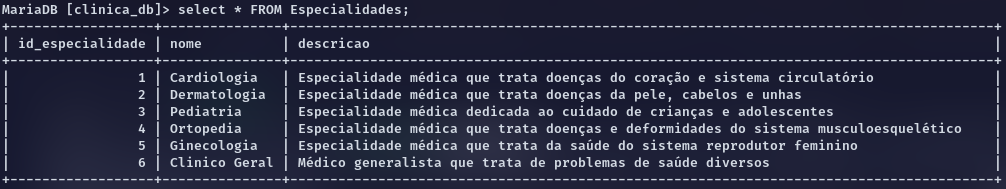
\includegraphics[width=1\linewidth]{Text/DML/Especialidades.png}
    \caption{Tabela Especialidades - \texttt{SELECT * FROM Especialidades;}}
    \label{fig:Especialidades}
\end{figure}

\begin{figure}[H]
    \centering
    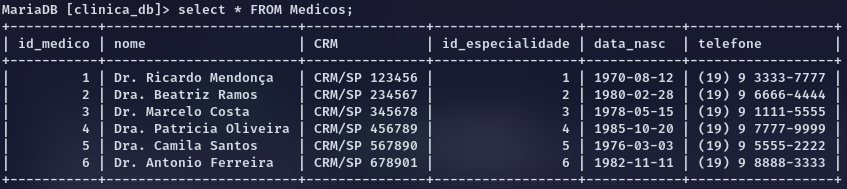
\includegraphics[width=1\linewidth]{Text/DML/Medicos.png}
    \caption{Tabela Medicos - \texttt{SELECT * FROM Medicos;}}
    \label{fig:Medicos}
\end{figure}

\begin{figure}[H]
    \centering
    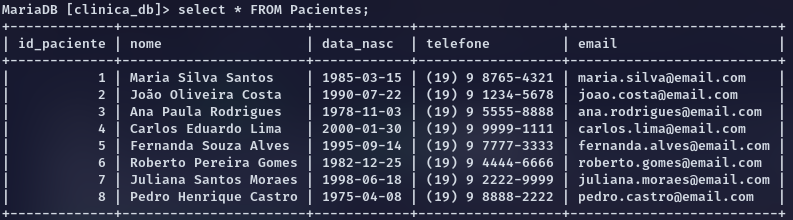
\includegraphics[width=1\linewidth]{Text/DML/Pacientes.png}
    \caption{Tabela Pacientes - \texttt{SELECT * FROM Pacientes;}}
    \label{fig:Pacientes}
\end{figure}

\begin{figure}[H]
    \centering
    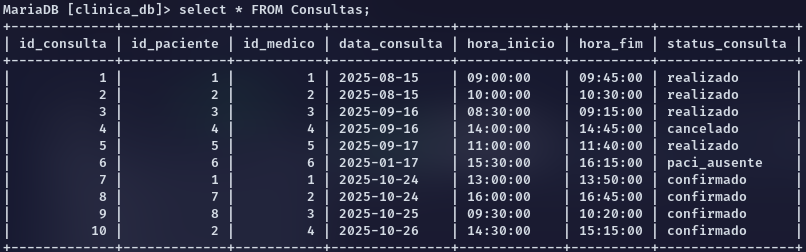
\includegraphics[width=1\linewidth]{Text/DML/Consultas.png}
    \caption{Tabela Consultas - \texttt{SELECT * FROM Consultas;}}
    \label{fig:Especialdiades}
\end{figure}

\begin{figure}[H]
    \centering
    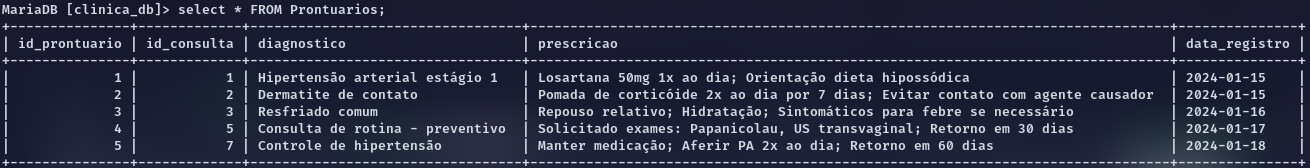
\includegraphics[width=1\linewidth]{Text/DML/Prontuarios.png}
    \caption{Tabela Prontuarios - \texttt{SELECT * FROM Prontuarios;}}
    \label{fig:Prontuarios}
\end{figure}

\newpage
\subsection{Procedimentos e Funções}\label{subsec:proc}
\begin{lstlisting}[
    language=MySQL,
    caption=Script para criação do procedimento \texttt{Agendar},
    label=AgendarProc
]
DELIMITER $$

CREATE PROCEDURE Agendar(
    IN p_id_paciente      INT,
    IN p_id_medico        INT,
    IN p_data_consulta    DATE,
    IN p_hora_inicio      TIME,
    IN p_hora_fim         TIME
)
BEGIN
DECLARE conflito_medico INT DEFAULT 0; 

-- Inicia a transacao
START TRANSACTION;

-- verifica data e hora sao validas
IF (p_data_consulta < CURDATE()
    OR
    p_data_consulta = CURDATE() AND p_hora_inicio < ADDTIME(CURTIME(), '01:00:00')
   ) THEN

    SIGNAL SQLSTATE '45000'
    SET MESSAGE_TEXT = 'Erro: Hora ou data nao validos!';
END IF;

-- Verifica conflito na agenda do medico
SELECT COUNT(*) INTO conflito_medico
FROM Consultas
WHERE id_medico = p_id_medico
    AND data_consulta = p_data_consulta
    AND status_consulta != 'cancelado' -- Ignora consultas canceladas
    AND ( 
        -- Conflito: nova consulta inicia durante uma existente
        (p_hora_inicio >= hora_inicio AND p_hora_inicio < hora_fim) 
        OR
        -- Conflito: nova consulta termina durante uma existente  
        (p_hora_fim > hora_inicio AND p_hora_fim <= hora_fim) 
        OR
        -- Conflito: nova consulta engloba uma existente
        (p_hora_inicio <= hora_inicio AND p_hora_fim >= hora_fim)
    );    

-- Na ausencia de conflitos:
IF conflito_medico = 0 THEN
    INSERT INTO Consultas 
        (id_paciente, id_medico, data_consulta, hora_inicio, hora_fim, status_consulta)
    VALUES
        (p_id_paciente, p_id_medico, p_data_consulta, p_hora_inicio, p_hora_fim, 'confirmado');

    COMMIT; -- Confirma a transicao
    
    SELECT 'Consulta agendada com sucesso!' AS Mensagem;
    SELECT * FROM Consultas WHERE 
        id_paciente=p_id_paciente AND 
        data_consulta = p_data_consulta AND 
        hora_inicio = p_hora_inicio;
    
ELSE -- Se conflito:
    ROLLBACK; -- Cancela as mudancas na transiction    
    
    SIGNAL SQLSTATE '45000'
    SET MESSAGE_TEXT = 'Erro: Medico ja possui uma consulta agendada nesse horario';
END IF;

END $$
DELIMITER ;
\end{lstlisting}